\documentclass{article}

\author{Pedro Henrique Limeira da Cruz}
\title{Resistência dos Materiais - I}

\usepackage[margin=0.8in]{geometry}
\usepackage{indentfirst}
\usepackage{fancyhdr}
\usepackage{tcolorbox} 
\usepackage{graphicx}
\usepackage{amsmath}
\usepackage{amssymb}
\usepackage{enumitem}
\usepackage{tabularx} % in the preamble


% Create a Todo list
\newlist{todolist}{itemize}{2}
\setlist[todolist]{label=$\square$}


% Create a new command to be used in the align environment in multiple line equations do only the last equation is numbered  
\newcommand{\n}{\nonumber \\ }
\makeatletter
\let\inserttitle\@title
\makeatother
% Set the style of the page 
\pagestyle{fancy}
\fancyhf{}
\rhead{Pedro Henrique L. da Cruz}
\lhead{\inserttitle}
\rfoot{Page \thepage}

\usepackage{hyperref}
\hypersetup{
    colorlinks=true,
    linkcolor=black,
    filecolor=magenta,
    urlcolor=cyan,
}

% Begin the Document 
\begin{document}

\maketitle
\thispagestyle{empty}

% Add the image inside a figure in as the first page
% \begin{figure}[h]
%     \begin{center}
%         
\includegraphics[scale = 0.15]{/Users/pedrocruz/Documents/UNICAMP/ES101/ES101 - Robotic Arm/img/unicamp.png}
%     \end{center}
% \end{figure}

% Change to the Next page 
\newpage
\tableofcontents
\newpage

\section{Introdução e Definições}

A matéria de resistência dos materiais que iremos estudar nada mais é do que a análise de mecânica estática, só que, dessa vez, para corpos que se deformam.
Levando isso em consideração, teremos primeiro que revisar alguns conceitos importantes de estática, sendo eles, de modo geral:
\begin{itemize}
    \item Modelos de Suporte e Vínculos
    \item Equilíbrio Estático : cargas simples, combinadas, carregamentos distribuídos, ...
\end{itemize}

\subsection{Modelos de Suporte e Vínculos}

Como o nosso objetivo é modelar o sistema para aplicarmos os equacionamentos de estática (e mais para frente outros mais específicos de ResMat) precisamos, primeiro, ser capazes de
identificar as forças que atuam sobre o corpo em análise. Por isso remos revisar as diferentes forças de reação que cada tipo de suporte gera em uma viga:

\begin{table}[h]
    \begin{tabular}{|l|c|c|c|l|l|}\hline
        \textbf{Nome}                                               & \textbf{Exemplo} & \textbf{Representação} & \textbf{D.C.L} & \textbf{Descrição} & \textbf{Cometário} \\ \hline

        Rolete                                                      &

        \begin{minipage}{.2\textwidth}
            \centering
            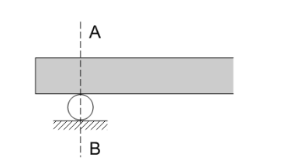
\includegraphics[width=\textwidth]{imgs/rolete_eg.png}
        \end{minipage}      &

        \begin{minipage}{.2\columnwidth}
            \centering
            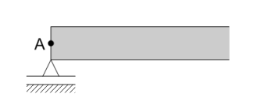
\includegraphics[width=\textwidth]{imgs/rolete_rep.png}
        \end{minipage}     &

        \begin{minipage}{.2\columnwidth}
            \centering
            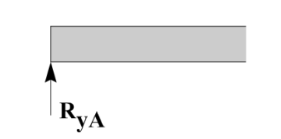
\includegraphics[width=.85\textwidth]{imgs/rolete_dcl.png}
        \end{minipage}  &

        \begin{minipage}{.1\columnwidth}
            \tiny
            •Resistente a forças em \emph{somente uma linha de direção}

            •Reação de apoio: 1 incógnita
        \end{minipage} &

        \begin{minipage}{.1\columnwidth}
            \vspace{5px}
            \tiny
            Importante observar que a representação possui \textbf{DUAS} linhas horzontais abaixo do triângulo.
            \vspace{5px}
        \end{minipage}                                                                 \\ \hline

        Pino                                                        &

        \begin{minipage}{.2\textwidth}
            \centering
            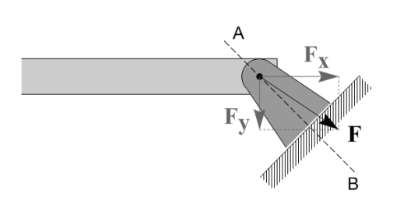
\includegraphics[width=\textwidth]{imgs/pino_eg.png}
        \end{minipage}        &

        \begin{minipage}{.2\columnwidth}
            \centering
            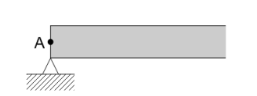
\includegraphics[width=\textwidth]{imgs/pino_rep.png}
        \end{minipage}       &

        \begin{minipage}{.2\columnwidth}
            \centering
            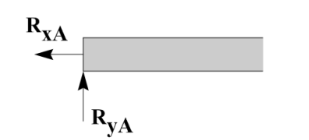
\includegraphics[width=\textwidth]{imgs/pino_dcl.png}
        \end{minipage}       &

        \begin{minipage}{.1\columnwidth}
            \tiny
            •Resistente a forças em \emph{duas linhas de ação}

            •Reação de apoio: 2 incógnitas
        \end{minipage}          &

        \begin{minipage}{.1\columnwidth}
            \vspace{5px}
            \tiny
            Importante observar que a representação possui somente \textbf{UMA} linha horzontai abaixo do triângulo.
            \vspace{5px}
        \end{minipage}                                                            \\ \hline


        Engaste                                                     &

        \begin{minipage}{.2\textwidth}
            \centering
            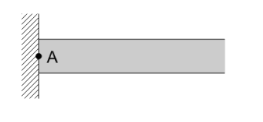
\includegraphics[width=\textwidth]{imgs/engaste_rep.png}
        \end{minipage}    &

        \begin{minipage}{.2\columnwidth}
            \centering
            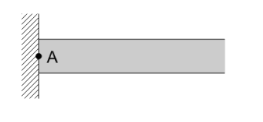
\includegraphics[width=\textwidth]{imgs/engaste_rep.png}
        \end{minipage}    &

        \begin{minipage}{.2\columnwidth}
            \centering
            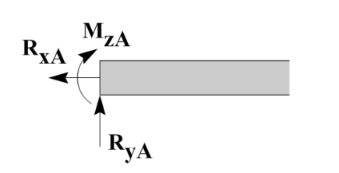
\includegraphics[width=\textwidth]{imgs/engaste_dcl.png}
        \end{minipage}    &

        \begin{minipage}{.1\columnwidth}
            \tiny
            • Resiste a \textbf{Forças} e \textbf{Momentos}
        \end{minipage}             &

        \begin{minipage}{.1\columnwidth}
            \vspace{5px}
            \tiny
            Até o momento é o único vínculo que resiste a momento.
            \vspace{5px}
        \end{minipage}                                                                                                              \\ \hline
    \end{tabular}
    \caption{Principais Suportes e Vínculos - 2D}
\end{table}

Tendo em vista que há diferentes suportes e vínculos, é importante entender o processo de escolha de vínculos durante análise de uma força/momento. Para tal, podemos nos perguntar:
\begin{enumerate}
    \item \textbf{O apoio/vínculo impede algum movimento que será resultante da força sob análise?} Se a resposta for \emph{não}, podemos simplesmente desconsiderar o vinculo na nossa
          modelagem. Se a resposta for \emph{sim}, ele impede um movimento, podemos prosseguir para outras perguntas.
    \item \textbf{O apoio/vínculo impede que a peça "gire" como resultado da força?} Se a resposta for \emph{sim} isso significa que o suporte restringe tanto forças quanto
          \emph{momentos}. Como temos somente um vínculo (o engaste) que tem essa característica, podemos usa-lo durante nossa modelagem. Se a resposta for não, ficamos entre um rolete e um pino.
    \item \textbf{O apoio/vínculo impede a movimentação, que seria resultante da força, em mais de um eixo?} Se \emph{sim}, temos um pino. Caso contrário teremos um rolete.
\end{enumerate}

\subsection{Equilíbrio Estático}

Como dito anteriormente, o ponto de partida de ResMat é a estática mecânica. Agora que já definimos os principais modelos de forças de reação, podemos descrever o equilíbrio estático
(assim como foi feito durante o estudo de Estática).

O principal conceito que rege o equilíbrio estático é que o sistema não possui aceleração, logo há a conservação tanto da quantidade de movimento linear quanto angular, resultando nas
respectivas equações:

$$\\$$

\begin{minipage}{.5\linewidth}
    \begin{align*}
        \sum \vec F = 0 \Rightarrow \begin{cases}
                                        \sum F_x = 0 \\
                                        \sum F_y = 0 \\
                                        \sum F_z = 0
                                    \end{cases}
    \end{align*}
\end{minipage}%
\begin{minipage}{.5\textwidth}
    \begin{align*}
        \sum \vec M = 0 \Rightarrow \begin{cases}
                                        \sum M_x = 0 \\
                                        \sum M_y = 0 \\
                                        \sum M_z = 0
                                    \end{cases}
    \end{align*}
\end{minipage}


$$\\$$

Para problemas de sistemas planos, as equações se resumem à:

$$\\$$

\begin{minipage}{.5\textwidth}
    \centering
    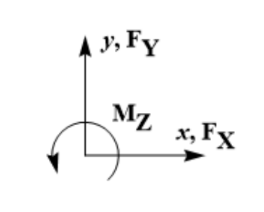
\includegraphics[width=.5\textwidth]{imgs/sis_plano.png}
\end{minipage}%
\begin{minipage}{.5\textwidth}
    \begin{align*}
        \sum F_x = 0 \\
        \sum F_y = 0 \\
        \sum M_z = 0
    \end{align*}
\end{minipage}

A depender da topologia, no que tange equilíbrio estático, um sistema pode ser definido como:
\begin{itemize}
    \item \textbf{Sistema Isostático}: As vinculações são suficientes para satisfazer o equilíbrio estático, número de incógnitas igual ao numero de equações.
    \item \textbf{Sistema Hiperestático}: As vinculações são em excesso para satisfazer o equilíbrio estático, número de incógnitas maior ao numero de equações.
    \item \textbf{Sistema Hipostático}: As vinculações não são suficientes para satisfazer o equilíbrio estático, número de incógnitas menor ao numero de equações.
\end{itemize}

\newpage
\subsection{Carregamentos Combinados}
Já vimos anteriormente no caso de cargas combinadas que, a depender das forças que o corpo sofre (e resiste) nós iremos representar os suportes e vínculos de uma forma específica.
Agora, nós iremos expandir esse assunto e descrever de forma detalhada os diferentes modelos que nós usamos para os corpos que sofrem essas forças e reações e descrever suas prioridades.

A parte mais fundamental para entender o porque há diferentes modelos para descrever os corpos que \textbf{são esbeltos} (\emph{i.e} possuem comprimento muito maior que sua largura e
altura) é:

$$\\$$
\begin{center}
    \textbf{Problemas de carregamento transversal, longitudinal e torsional são independentes}
\end{center}
$$\\$$

Isso nos diz que podem haver problemas de carregamentos combinados que sejam necessários 3 modelos distintos para serem modelados, cada um com um modelo específico para o corpo, como
podemos ver abaixo:

\begin{table}[h]
    \centering
    \begin{tabular}{|l|c|l|c|}\hline
        \textbf{Nome} & \textbf{Exemplo} & \textbf{Descrição} & \textbf{Equação} \\ \hline
        Barra
                      &
        \begin{minipage}{.4\textwidth}
            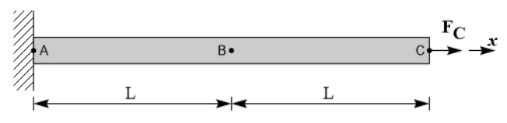
\includegraphics[width=\textwidth]{imgs/barra_eg.png}
        \end{minipage}
                      &
        \begin{minipage}{.3\textwidth}
            Corpos sujeitos \textbf{somente a cargas logitudinais/axiais}
        \end{minipage}
                      &
        $\sum F_x = 0$                                                           \\ \hline

        Eixo
                      &
        \begin{minipage}{.4\textwidth}
            \vspace{10px}
            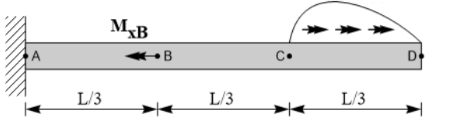
\includegraphics[width=.9\textwidth]{imgs/eixo_eg.png}
        \end{minipage}
                      &
        \begin{minipage}{.3\textwidth}
            Corpos sujeitos \textbf{somente a cargas torcionais}
        \end{minipage}
                      &
        $\sum M_x = 0$                                                           \\ \hline
        Viga
                      &
        \begin{minipage}{.4\textwidth}
            \vspace{10px}
            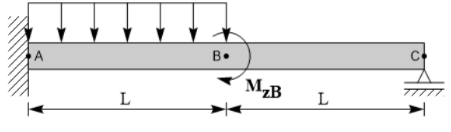
\includegraphics[width=.9\textwidth]{imgs/viga_eg.png}
        \end{minipage}
                      &
        \begin{minipage}{.3\textwidth}
            Corpos sujeitos \textbf{somente a cargas transversais e/ou momentos fletores}
        \end{minipage}
                      &
        $\sum M_z,F_y = 0$                                                       \\ \hline
    \end{tabular}
    \caption{Tabela de Modelos para Corpos Esbeltos}
\end{table}

\newpage
\subsection{Equilíbrio Interno de Corpos}
Para começarmos a entrar no assunto de deformação dos corpos, é primeiro necessário entender que quando há o \textbf{equilíbrio estático de um corpo}, há também um \textbf{equilíbrio entre quaisquer duas
    partes internas} do corpo, que \textbf{sofrem esforços internos}, sendo eles:
\begin{itemize}
    \item Esforços Axial $N_x(x)$
    \item Esforço Cortante $V_y(x)$
    \item Momento Fletor $M_z(x)$
    \item Momento Torsor $M_x(x)$
\end{itemize}

\subsubsection{Convenção de Sinais}
Quando estivermos lidando com a análise de esforços internos e deformações de corpos, nós iremos seguir a seguinte convenção de sinais:
\begin{figure}[h]
    \centering
    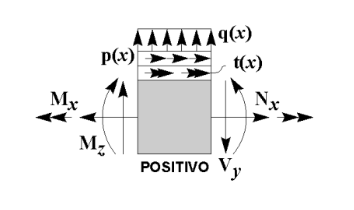
\includegraphics[width=.3\textwidth]{imgs/conv_sinais.png}
    \caption{Convenção de Sinais para Esforços Internos}
    \label{fig:conv_de_sinais_esf_intern}
\end{figure}


A partir dessa convenção e da análise dos momentos fletores $M_z$ e esforços cortantes $V_x$ conhecidos nós somos capazes de analisar a deformação de um corpo esbelto (\emph{e.g} uma viga),
como mostrado abaixo:
\begin{figure}[h]
    \centering
    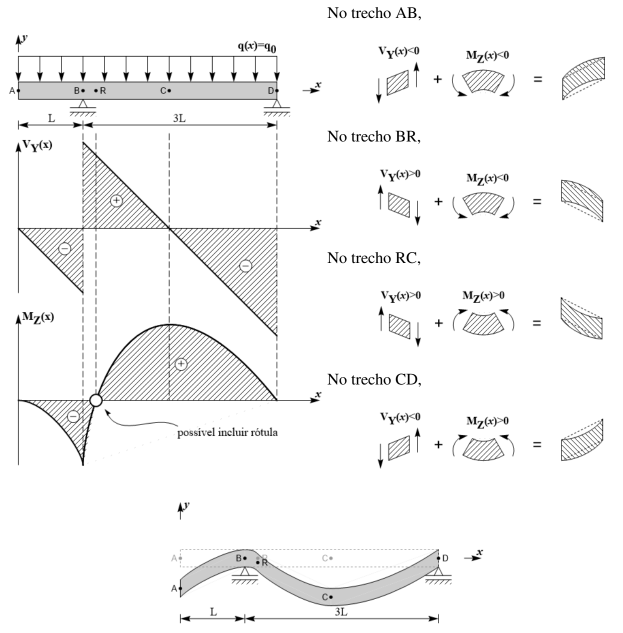
\includegraphics[width=.55\textwidth]{imgs/conv_sinais_eg.png}
    \caption{Exemplo de Análise de Forças Internas e Deformação}
\end{figure}

\subsection{One Pager - Introdução e Definições}
Modelo de Suportes:
\begin{table}[h]\tiny
    \begin{tabularx}{\textwidth}{|l|X|X|X|l|l|}\hline
        \textbf{Nome}                                               & \textbf{Exemplo} & \textbf{Representação} & \textbf{D.C.L} & \textbf{Descrição} & \textbf{Cometário} \\ \hline

        Rolete                                                      &

        \begin{minipage}{.2\textwidth}
            \centering
            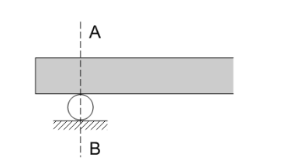
\includegraphics[width=.8\textwidth]{imgs/rolete_eg.png}
        \end{minipage}    &

        \begin{minipage}{.2\columnwidth}
            \centering
            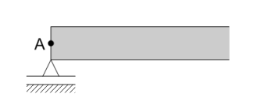
\includegraphics[width=.8\textwidth]{imgs/rolete_rep.png}
        \end{minipage}   &

        \begin{minipage}{.2\columnwidth}
            \centering
            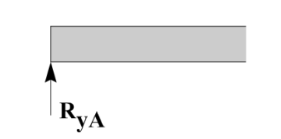
\includegraphics[width=.8\textwidth]{imgs/rolete_dcl.png}
        \end{minipage}   &

        \begin{minipage}{.1\columnwidth}
            \tiny
            •Resistente a forças em \emph{somente uma linha de direção}

            •Reação de apoio: 1 incógnita
        \end{minipage} &

        \begin{minipage}{.1\columnwidth}
            \vspace{5px}
            \tiny
            Importante observar que a representação possui \textbf{DUAS} linhas horzontais abaixo do triângulo.
            \vspace{5px}
        \end{minipage}                                                                 \\ \hline

        Pino                                                        &

        \begin{minipage}{.2\textwidth}
            \centering
            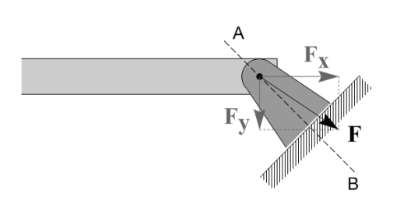
\includegraphics[width=.8\textwidth]{imgs/pino_eg.png}
        \end{minipage}      &

        \begin{minipage}{.2\columnwidth}
            \centering
            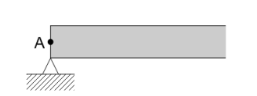
\includegraphics[width=.8\textwidth]{imgs/pino_rep.png}
        \end{minipage}     &

        \begin{minipage}{.2\columnwidth}
            \centering
            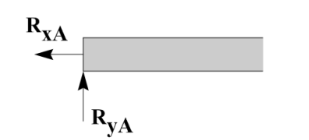
\includegraphics[width=.8\textwidth]{imgs/pino_dcl.png}
        \end{minipage}     &

        \begin{minipage}{.1\columnwidth}
            \tiny
            •Resistente a forças em \emph{duas linhas de ação}

            •Reação de apoio: 2 incógnitas
        \end{minipage}          &

        \begin{minipage}{.1\columnwidth}
            \vspace{5px}
            \tiny
            Importante observar que a representação possui somente \textbf{UMA} linha horzontai abaixo do triângulo.
            \vspace{5px}
        \end{minipage}                                                            \\ \hline


        Engaste                                                     &

        \begin{minipage}{.2\textwidth}
            \centering
            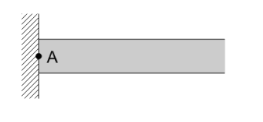
\includegraphics[width=.8\textwidth]{imgs/engaste_rep.png}
        \end{minipage}  &

        \begin{minipage}{.2\columnwidth}
            \centering
            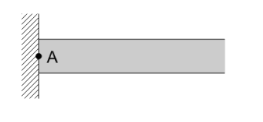
\includegraphics[width=.8\textwidth]{imgs/engaste_rep.png}
        \end{minipage}  &

        \begin{minipage}{.2\columnwidth}
            \centering
            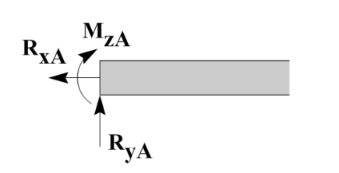
\includegraphics[width=.8\textwidth]{imgs/engaste_dcl.png}
        \end{minipage}  &

        \begin{minipage}{.1\columnwidth}
            \tiny
            • Resiste a \textbf{Forças} e \textbf{Momentos}
        \end{minipage}             &

        \begin{minipage}{.1\columnwidth}
            \vspace{5px}
            \tiny
            Até o momento é o único vínculo que resiste a momento.
            \vspace{5px}
        \end{minipage}                                                                                                              \\ \hline
    \end{tabularx}
\end{table}

\begin{minipage}{.9\textwidth}\tiny
    \begin{enumerate}
        \item \textbf{O apoio/vínculo impede algum movimento que será resultante da força sob análise?} Se a resposta for \emph{não}, podemos simplesmente desconsiderar o vinculo na nossa
              modelagem. Se a resposta for \emph{sim}, ele impede um movimento, podemos prosseguir para outras perguntas.
        \item \textbf{O apoio/vínculo impede que a peça "gire" como resultado da força?} Se a resposta for \emph{sim} isso significa que o suporte restringe tanto forças quanto
              \emph{momentos}. Como temos somente um vínculo (o engaste) que tem essa característica, podemos usa-lo durante nossa modelagem. Se a resposta for não, ficamos entre um rolete e um pino.
        \item \textbf{O apoio/vínculo impede a movimentação, que seria resultante da força, em mais de um eixo?} Se \emph{sim}, temos um pino. Caso contrário teremos um rolete.
    \end{enumerate}
\end{minipage}

$$\\$$

Equilíbrio Estático e Definição:

\begin{minipage}{.4\textwidth}\small
    \begin{align*}
        \sum F_x = 0 \\
        \sum F_y = 0 \\
        \sum M_z = 0
    \end{align*}
\end{minipage}%
\begin{minipage}{.6\textwidth}\tiny
    \begin{itemize}
        \item \textbf{Sistema Isostático}: As vinculações são suficientes para satisfazer o equilíbrio estático, número de incógnitas igual ao numero de equações.
        \item \textbf{Sistema Hiperestático}: As vinculações são em excesso para satisfazer o equilíbrio estático, número de incógnitas maior ao numero de equações.
        \item \textbf{Sistema Hipostático}: As vinculações não são suficientes para satisfazer o equilíbrio estático, número de incógnitas menor ao numero de equações.
    \end{itemize}
\end{minipage}

$$\\$$

Carregamentos Combinados e Modelos de Corpos Esbeltos:
\begin{table}[h]\tiny
    \centering
    \begin{tabularx}{\textwidth}{|l|X|l|X|}\hline
        \textbf{Nome} & \textbf{Exemplo} & \textbf{Descrição} & \textbf{Equação} \\ \hline
        Barra
                      &
        \begin{minipage}{.4\textwidth}
            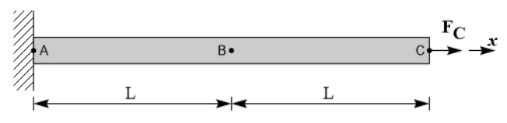
\includegraphics[width=.5\textwidth]{imgs/barra_eg.png}
        \end{minipage}
                      &
        Corpos sujeitos \textbf{somente a cargas logitudinais/axiais}
                      &
        $\sum F_x = 0$                                                           \\ \hline

        Eixo
                      &
        \begin{minipage}{.4\textwidth}
            \vspace{10px}
            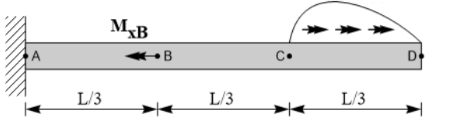
\includegraphics[width=.5\textwidth]{imgs/eixo_eg.png}
        \end{minipage}
                      &
        Corpos sujeitos \textbf{somente a cargas torcionais}
                      &
        $\sum M_x = 0$                                                           \\ \hline
        Viga
                      &
        \begin{minipage}{.4\textwidth}
            \vspace{10px}
            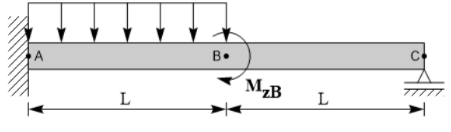
\includegraphics[width=.5\textwidth]{imgs/viga_eg.png}
        \end{minipage}
                      &
        Corpos sujeitos \textbf{somente a cargas transversais e/ou momentos fletores}
                      &
        $\sum M_z,F_y = 0$                                                       \\ \hline
    \end{tabularx}
\end{table}

$$\\$$

Convenção De Sinais - Esforços Internos:

\begin{minipage}{.5\textwidth}
    \centering
    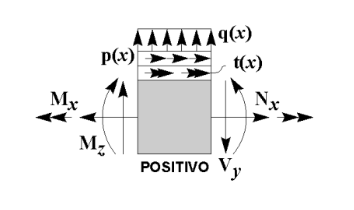
\includegraphics[width=.7\textwidth]{imgs/conv_sinais.png}
\end{minipage}%
\begin{minipage}{.5\textwidth}\tiny
    \begin{itemize}
        \item Esforços Axial $N_x(x)$
        \item Esforço Cortante $V_y(x)$
        \item Momento Fletor $M_z(x)$
        \item Momento Torsor $M_x(x)$
    \end{itemize}
\end{minipage}

\newpage

\section{Método das Equações Diferenciais de Equilíbrio}
\subsection{Introdução e Equações Diferenciais}
Até o momento nós vimos que se tivermos o esforço cortante e o momento fletor para um corpo nós somos capazes de deduzir a deformação. Agora, entretanto, iremos ver como que nós calculamos
esses valores para um corpo sofrendo carregamento. O nome do método para tal é o \textbf{Método das Equações Diferenciais}, onde nós relacionamos cada tipo de load externo (para barras,
vigas e eixos) com as respectivas reações internas, em um cenário diferencial (para uma parte infinitesimal do corpo de cada vez, para todo o corpo), como mostrado na tabela abaixo:

\begin{table}[h]
    \centering
    \begin{tabular}{|l|c|l|}\hline
        \textbf{Cenário}                      & \textbf{Equação}                                   & \textbf{Descrição}                                       \\ \hline
        \rule{0pt}{4ex} Barras                & $\frac{d}{dx}N_x(x) = -p(x)$                       & Onde $-p(x)$ é o carregamento longitudinal sendo sofrido \\[2ex]  \hline
        \rule{0pt}{4ex} Eixos                 & $\frac{d}{dx}M_x(x) = -t(x)$                       & Onde $-t(x)$ é o momento axial sofrido                   \\[2ex]\hline
        \rule{0pt}{4ex} Vigas: Cortante       & $\frac{d}{dx}V_y(x) = +q(x)$                       & Onde $+q(x)$ é o carregamento transversal sofrido        \\[2ex] \hline
        \rule{0pt}{4ex} Vigas: Momento Fletor & $\frac{d^2}{dx^2}M_z = \frac{d}{dx}V_y(x) = +q(x)$ & Onde $+q(x)$ é o carregamento transversal sofrido        \\[2ex] \hline
    \end{tabular}
    \caption{EDOs para principais modelos de corpos esbeltos}
    \label{tb:edo_esf_internos}
\end{table}

Relembrando, onde:
\begin{itemize}
    \item Esforços Axial $N_x(x)$
    \item Esforço Cortante $V_y(x)$
    \item Momento Fletor $M_z(x)$
    \item Momento Torsor $M_x(x)$
\end{itemize}

\newpage
\subsection{Condições de Contorno}
Se lembrarmos bem de calculo 3 e de equações diferenciais, todas as EDOs de grau $n$ precisam de $n$ pontos conhecidos para possam ser resolvidos, onde eles podem ser Pontos de
Contorno ou Condições Iniciais. Para o nosso caso, iremos estudar problemas com condições de contorno.

Para ser considerado uma condição de contorno é necessário:
\begin{enumerate}
    \item Estar Definida no Contorno do modelo
    \item Ser Conhecida a Priori
    \item Ser Relevante para o Problema
\end{enumerate}

Indo além, para os nosso problemas, 99\% das vezes as condições de contorno estarão em vínculos localizados nas extremidades do corpo sendo estudado (\emph{e.g} em uma ponta de uma viga). Iremos abaixo
\textbf{descrever as condições de contorno para os principais vínculos/apoios QUANDO PRESENTES NAS EXTREMIDADES DO CORPO}\footnote{Como estamos lidando com análise no eixo $x$, somente
    os vínculos que estão localizados nas extremidades (em $x=0$ ou $x=L$) são possíveis condições de contorno}.

\begin{table}[h]
    \centering
    \begin{tabular}{|l|c|l|}\hline
        \textbf{Vínculo}               & \textbf{Equações} & \textbf{Observações}                                                                                                          \\ \hline
        Extremidade Livre              &
        \begin{minipage}{.4\textwidth}
            {\begin{align*}
                     & \sum M_x, M_z = 0 \\
                     & \sum N_x, V_y = 0
                \end{align*}}
        \end{minipage} &

        \begin{minipage}{.4\textwidth}
            \vspace{5px}
            Como uma extremidade livre não apresenta reação a força nem momento, \textbf{se não for dito que há um valor diferente} para tais, na extremidade em questão os valores serão zero.
        \end{minipage} \\ \hline

        Rolete                         &
        \begin{minipage}{.4\textwidth}
            {\begin{align*}
                     & \sum M_x, M_z = 0 \\
                     & \sum N_x = 0
                \end{align*}}
        \end{minipage} &

        \begin{minipage}{.4\textwidth}
            \vspace{5px}
            Como um rolete não apresenta reação a momento, \textbf{se não for dito que há um valor diferente}, na extremidade em questão  o momento é zero (condição de contorno).
        \end{minipage}              \\ \hline

        Pino                           &
        \begin{minipage}{.4\textwidth}
            {\begin{align*}
                     & \sum M_z = 0
                \end{align*}}
        \end{minipage} &

        \begin{minipage}{.4\textwidth}
            \vspace{5px}
            Como um rolete não apresenta reação a momento, \textbf{se não for dito que há um valor diferente}, na extremidade em questão o momento é zero (condição de contorno).
        \end{minipage}               \\ \hline
    \end{tabular}
    \caption{Condições de Contorno para cada Vínculo}
    \label{tb:cond_contorno}
\end{table}

\newpage
\subsection{Função de Singularidade}
Até o momento vimos que podemos modelar os esforços e momentos interno de um corpo por equações diferenciais (como visto na tabela \ref{tb:edo_esf_internos}), e que para resolve-las
nós precisamos de condições de contorno (como visto na tabela \ref{tb:cond_contorno}). Antes de podermos resolver tais EDOs, entretanto, nós precisamos descrever os carregamentos
externos que o corpo está sofrendo (que seriam os membros do lado direito das EDOs).

Para casos em que os carregamentos são contínuos tal tarefa é extremamente fácil, só igualar a EDO ao valor (ou equação contínua) para todo $x$. Para os casos em que os carregamentos não são contínuos, entretanto, isso não é tão simples.

Para casos onde o carregamento não é contínuo, nós usaremos uma notação que simplifica toda a matemática complexa chamada de \textbf{Função de Singularidade}, onde:

\begin{align}
    \langle x - a\rangle^m = \begin{cases}
                                 0       & x<a     \\
                                 (x-a)^m & x \ge a
                             \end{cases}
    \label{eq:func_singularidade}
\end{align}

Onde a porção $\langle x - a \rangle$ rege a partir de qual ponto para de ser zero e o expoente $m$ rege o comportamento da curva a partir desse ponto, como mostra a figura abaixo:

\begin{table}[h]
    \centering
    \begin{tabular}{|c|c|l|} \hline
        \textbf{F. de Singularidade}                                   & \textbf{Gráfico} & \textbf{Use Cases}                                                             \\ \hline
        $\langle x - a\rangle^0$                                       &
        \begin{minipage}{.3\textwidth}
            \centering
            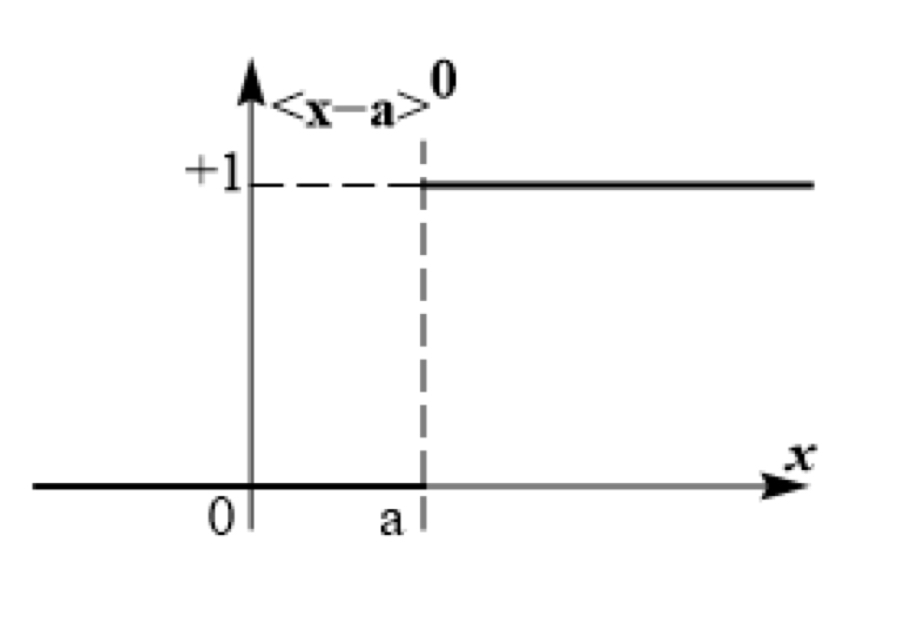
\includegraphics[width=.8\textwidth]{imgs/func_singul_0.jpeg}
        \end{minipage}  &
        \begin{minipage}{.4\textwidth}
            Usado mais durante análise de Vigas, quando há um carregamento de forças transversais para somente um intervalo da viga (\emph{e.g} de $L/2 \le x \le L$). Podemos,
            ainda, subtrair dois com um shift para ter um intervalo entre $a$ e $b$, como: $\langle x - a\rangle^0 - \langle x - b\rangle^0$
        \end{minipage} \\ \hline

        $\langle x - a\rangle^1$                                       &
        \begin{minipage}{.3\textwidth}
            \centering
            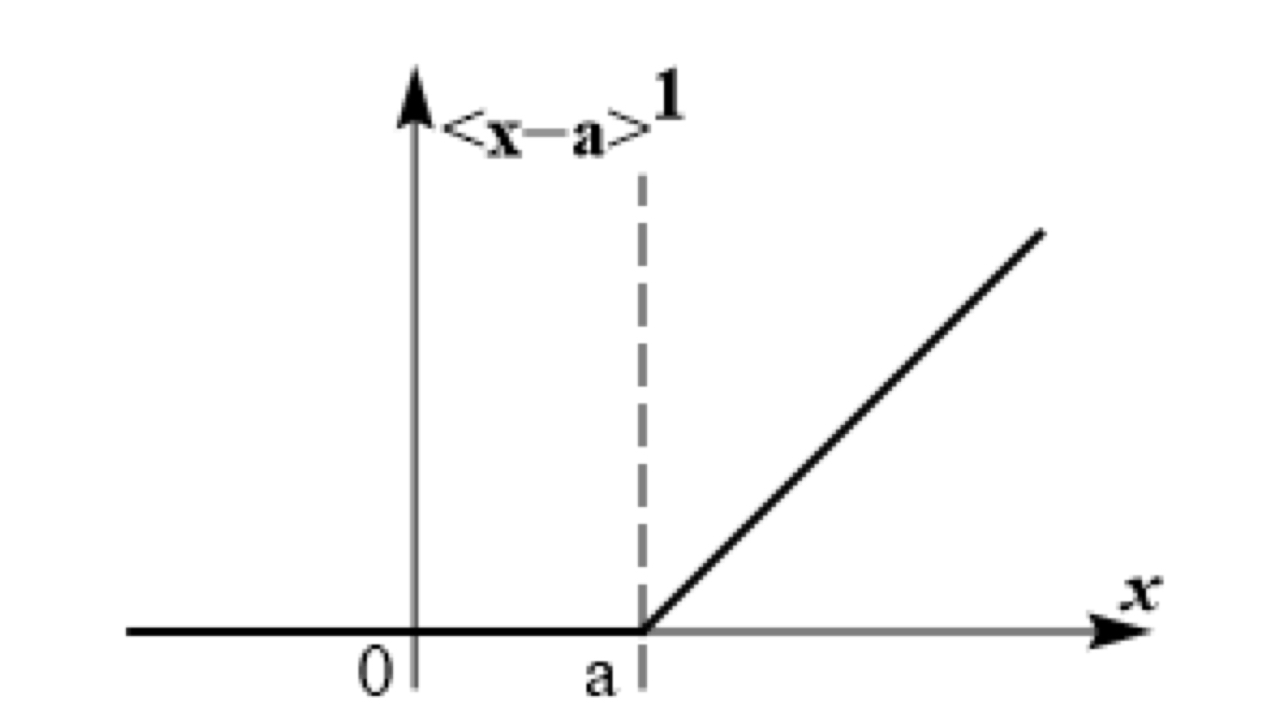
\includegraphics[width=.7\textwidth]{imgs/func_singul_1.jpeg}
        \end{minipage}  &
        \begin{minipage}{.4\textwidth}
            Também usado mais para análise de carregamento de vigas, mas nesse caso a força é zero até certo ponto $a$ e depois segue uma distribuição linear.
        \end{minipage}                  \\ \hline

        $\langle x - a\rangle^2$                                       &
        \begin{minipage}{.3\textwidth}
            \centering
            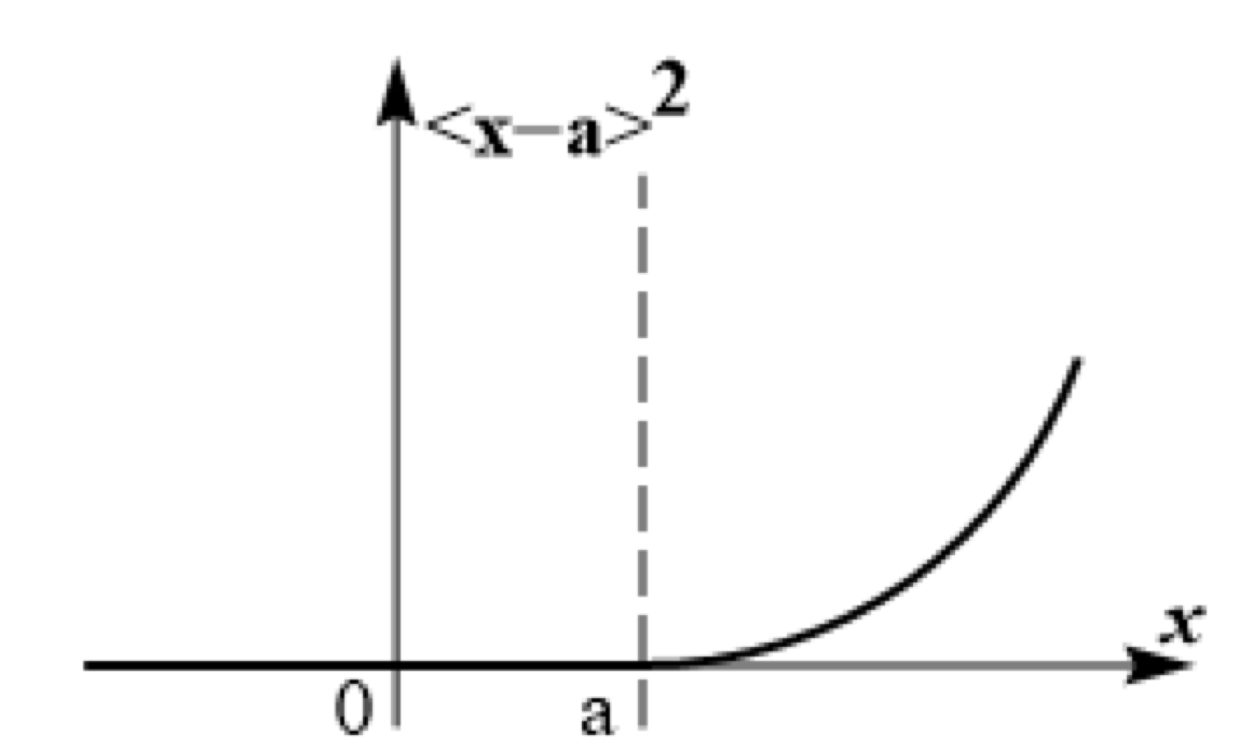
\includegraphics[width=.7\textwidth]{imgs/func_singul_2.jpeg}
        \end{minipage}  &
        \begin{minipage}{.4\textwidth}
            Também usado mais para análise de carregamento de vigas, mas nesse caso a força é zero até certo ponto $a$ e depois segue uma distribuição quadrática.
        \end{minipage}              \\ \hline

        $\langle x - a\rangle^{-1}$                                    &
        \begin{minipage}{.3\textwidth}
            \centering
            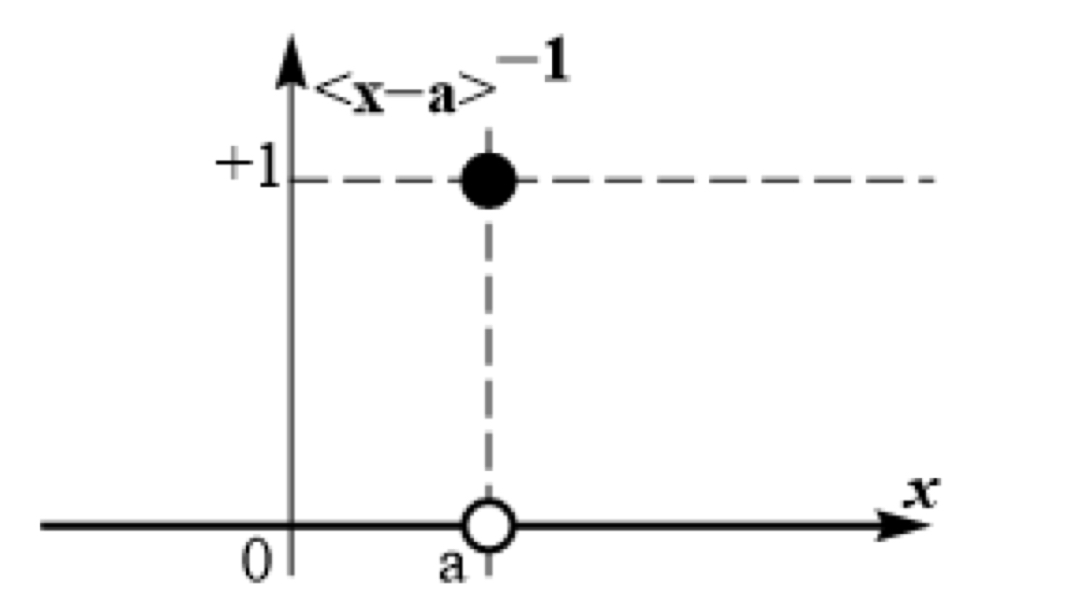
\includegraphics[width=.7\textwidth]{imgs/func_singul_-1.jpeg}
        \end{minipage} &
        \begin{minipage}{.4\textwidth}
            Usando bastante para representar forças pontuais durante análise de vigas, mas também usada para representar momentos durante análise de eixos.
        \end{minipage}                     \\ \hline

        $\langle x - a\rangle^{-2}$                                    &
        \begin{minipage}{.3\textwidth}
            \centering
            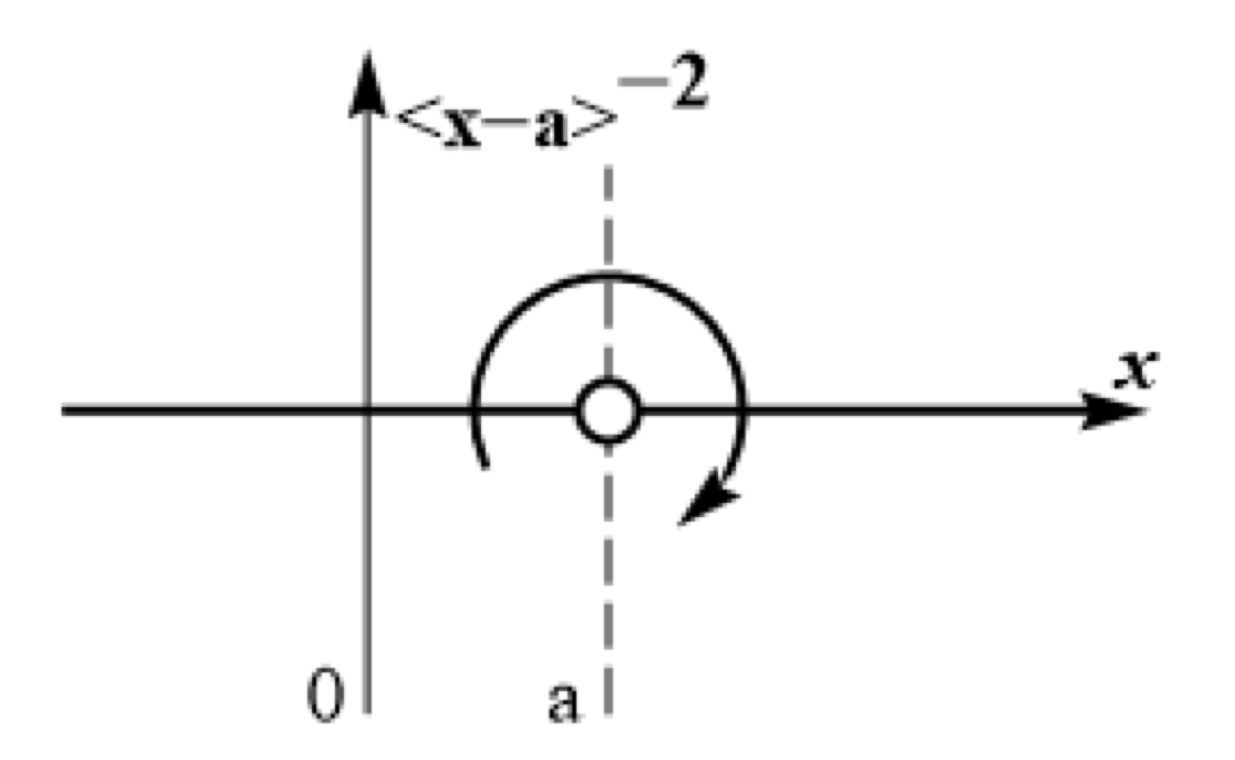
\includegraphics[width=.7\textwidth]{imgs/func_singul_-2.jpeg}
        \end{minipage} &
        \begin{minipage}{.4\textwidth}
            Usado bastante durante análise de vigas para representar momentos fletores.
        \end{minipage}                                                                                         \\ \hline
    \end{tabular}
\end{table}

Além disso, é importante entendermos o comportamento das funções de singularidade em relação a integração:
\begin{align*}
    \int \langle x-a\rangle^m dx    & = \frac{\langle x - a \rangle ^{m+1}}{m + 1}, m \ge 0 \\
    \int \langle x-a\rangle^{-1} dx & = \langle x - a \rangle^0                             \\
    \int \langle x-a\rangle^{-2} dx & = \langle x - a \rangle^{-1}                          \\
\end{align*}

\subsection{Método de Resolução - Equações Diferenciais de Equilíbrio}
Já vimos quais EDOs são aplicáveis para cada modelo, os possíveis valores de contorno e também como modelar as cargas externas sendo aplicadas, o que nos resta agora é saber como
juntar todos esses dados em um problema para resolve-lo. Para isso, nós vamos seguir 7 passos, como mostrado abaixo:
\begin{enumerate}\addtocounter{enumi}{-1}%
    \item Separar Carregamentos externos que são separáveis em seus respectivos modelos (barra, eixo, viga).
    \item Estabelecer uma convenção de sinais: A fim de padronizar, seguir a convenção da figura \ref{fig:conv_de_sinais_esf_intern}
    \item Estabelecer uma equação diferencial: A partir da tabela \ref{tb:edo_esf_internos}
    \item Descrever condições de Contorno e Restrição: Bom indicativo é começar pelos da tabela \ref{tb:cond_contorno} + Comportamento de Rótulas
    \item Integrar a equação diferencial: Como mostrado na subsection anterior
    \item Determinar Constantes de Integração: Substituindo os valores de contorno (já que são os únicos pontos conhecidos)
\end{enumerate}

Temos, ainda, algumas observações que podem ajudar a fazer os exercícios:
\begin{itemize}
    \item Se há uma carga distribuída que é aplicada sobre um possível ponto de contorno (\emph{e.g} como uma extremidade livre de um eixo engastado) por ela ser DISTRIBUÍDA, em um só
          ponto ela é igual a zero logo A CONDIÇÃO DE CONTORNO AINDA É VÁLIDA. Então se for uma extremidade livre, mesmo com um momento torsor distribuído sendo aplicado, no ponto ele é zero.
    \item Durante a modelagem dos valores de contorno, é importante ressaltar que eles seguem as convenções de sinais da figura \ref{fig:conv_de_sinais_esf_intern}, já para a modelagem da
          carga externa de momento fletor (não localizada nas extremidades) é positivo no sentido horário (como mostrado na imagem representativo da tabela das funções de singularidade).
    \item NÃO se bota no equacionamento de cargas os valores dos pontos de contorno.
    \item Quando for esboçar o gráfico lembraer que:
          \subitem $\square$ Quando for esboçar um intervalo, lembre de literalmente riscar partes que não são aplicáveis (para evitar que você calcule);
          \subitem $\square$ Antes de tentar esboçar um intervalo, simplifique o máximo possível (em função de $x$ mesmo, é mais fácil);
          \subitem $\square$ Substitua o valor inicial do intervalo somente no final da análise da seção, para saber a partir de qual ponto a seção começa, mas simplifique a equação SEM substituir valores.
\end{itemize}

\newpage
\subsection{One Pager - Método das Equação Diferencias de Equilíbrio}

Equações Diferenciais por Modelo de Corpo Esbelto:

\begin{table}[h]\tiny

    \begin{tabularx}{\textwidth}{|X|X|X|}\hline
        \textbf{Cenário}                         & \textbf{Equação}                                   & \textbf{Descrição}                                       \\ \hline
        \rule{0pt}{4ex} Barras - Esforço Axial   & $\frac{d}{dx}N_x(x) = -p(x)$                       & Onde $-p(x)$ é o carregamento longitudinal sendo sofrido \\[2ex]  \hline
        \rule{0pt}{4ex} Eixos - Momento Torsor   & $\frac{d}{dx}M_x(x) = -t(x)$                       & Onde $-t(x)$ é o momento axial sofrido                   \\[2ex]\hline
        \rule{0pt}{4ex} Vigaa - Esforço Cortante & $\frac{d}{dx}V_y(x) = +q(x)$                       & Onde $+q(x)$ é o carregamento transversal sofrido        \\[2ex] \hline
        \rule{0pt}{4ex} Vigas - Momento Fletor   & $\frac{d^2}{dx^2}M_z = \frac{d}{dx}V_y(x) = +q(x)$ & Onde $+q(x)$ é o carregamento transversal sofrido        \\[2ex] \hline
    \end{tabularx}

\end{table}
Condição de Contorno:



\begin{table}[h]
    \tiny
    \centering
    \begin{tabularx}{\textwidth}{|X|X|X|}\hline
        \textbf{Vínculo}               & \textbf{Equações} & \textbf{Observações}                                                                                                          \\ \hline
        Extremidade Livre              &
        \begin{minipage}{.3\textwidth}
            {\begin{align*}
                     & \sum M_x, M_z = 0 \\
                     & \sum N_x, V_y = 0
                \end{align*}}
        \end{minipage} &

        \begin{minipage}{.3\textwidth}
            \vspace{5px}
            Como uma extremidade livre não apresenta reação a força nem momento, \textbf{se não for dito que há um valor diferente} para tais, na extremidade em questão os valores serão zero.
        \end{minipage} \\ \hline

        Rolete                         &
        \begin{minipage}{.3\textwidth}
            {\begin{align*}
                     & \sum M_x, M_z = 0 \\
                     & \sum N_x = 0
                \end{align*}}
        \end{minipage} &

        \begin{minipage}{.3\textwidth}
            \vspace{5px}
            Como um rolete não apresenta reação a momento, \textbf{se não for dito que há um valor diferente}, na extremidade em questão  o momento é zero (condição de contorno).
        \end{minipage}              \\ \hline

        Pino                           &
        \begin{minipage}{.3\textwidth}
            {\begin{align*}
                    \sum M_z = 0
                \end{align*}}
        \end{minipage} &

        \begin{minipage}{.3\textwidth}
            \vspace{5px}
            Como um rolete não apresenta reação a momento, \textbf{se não for dito que há um valor diferente}, na extremidade em questão o momento é zero (condição de contorno).
        \end{minipage}               \\ \hline
    \end{tabularx}
\end{table}

\begin{todolist}\tiny
    \item Estar Definida no Contorno do modelo
    \item Ser Conhecida a Priori
    \item Ser Relevante para o Problema
\end{todolist}

Definição de Função de Singularidade:
\begin{table}[h]
    \tiny
    \centering
    \begin{tabularx}{\textwidth}{|X|X|l|}\hline
        \textbf{F. de Singularidade}                                   & \textbf{Gráfico} & \textbf{Use Cases}                                                             \\ \hline
        $\langle x - a\rangle^0$                                       &
        \begin{minipage}{.3\textwidth}
            \centering
            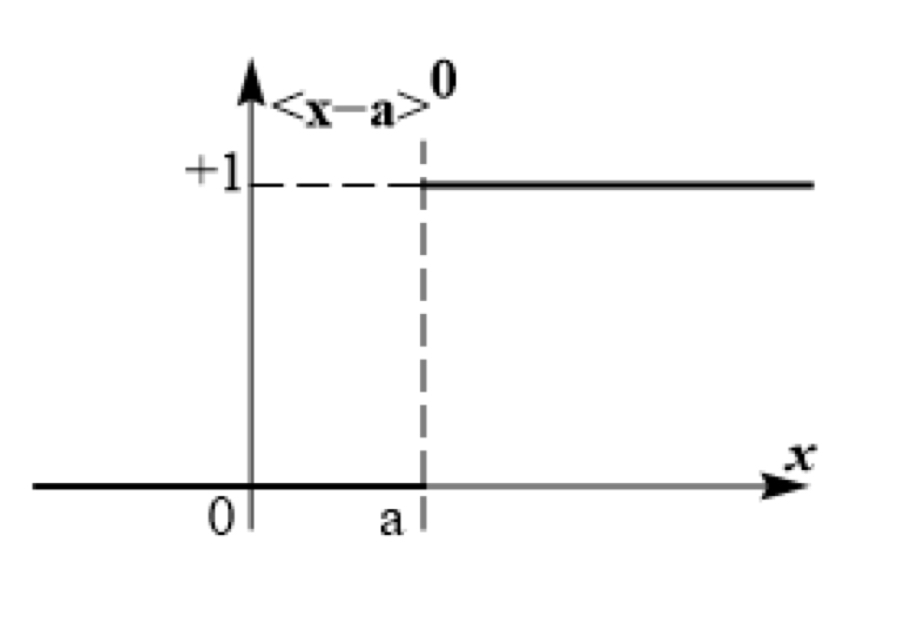
\includegraphics[width=.3\textwidth]{imgs/func_singul_0.jpeg}
        \end{minipage}  &
        \begin{minipage}{.4\textwidth}
            Usado mais durante análise de Vigas, quando há um carregamento de forças transversais para somente um intervalo da viga (\emph{e.g} de $L/2 \le x \le L$). Podemos,
            ainda, subtrair dois com um shift para ter um intervalo entre $a$ e $b$, como: $\langle x - a\rangle^0 - \langle x - b\rangle^0$
        \end{minipage} \\ \hline

        $\langle x - a\rangle^1$                                       &
        \begin{minipage}{.3\textwidth}
            \centering
            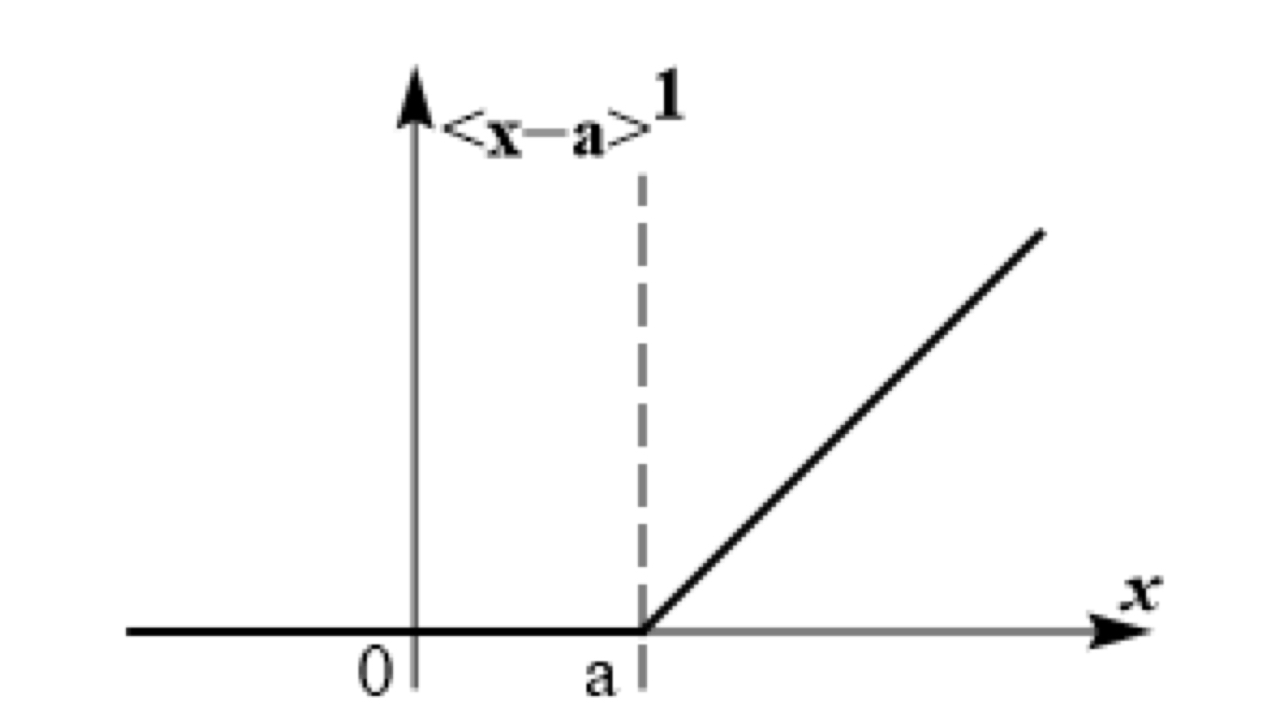
\includegraphics[width=.3\textwidth]{imgs/func_singul_1.jpeg}
        \end{minipage}  &
        \begin{minipage}{.4\textwidth}
            Também usado mais para análise de carregamento de vigas, mas nesse caso a força é zero até certo ponto $a$ e depois segue uma distribuição linear.
        \end{minipage}                  \\ \hline

        $\langle x - a\rangle^2$                                       &
        \begin{minipage}{.3\textwidth}
            \centering
            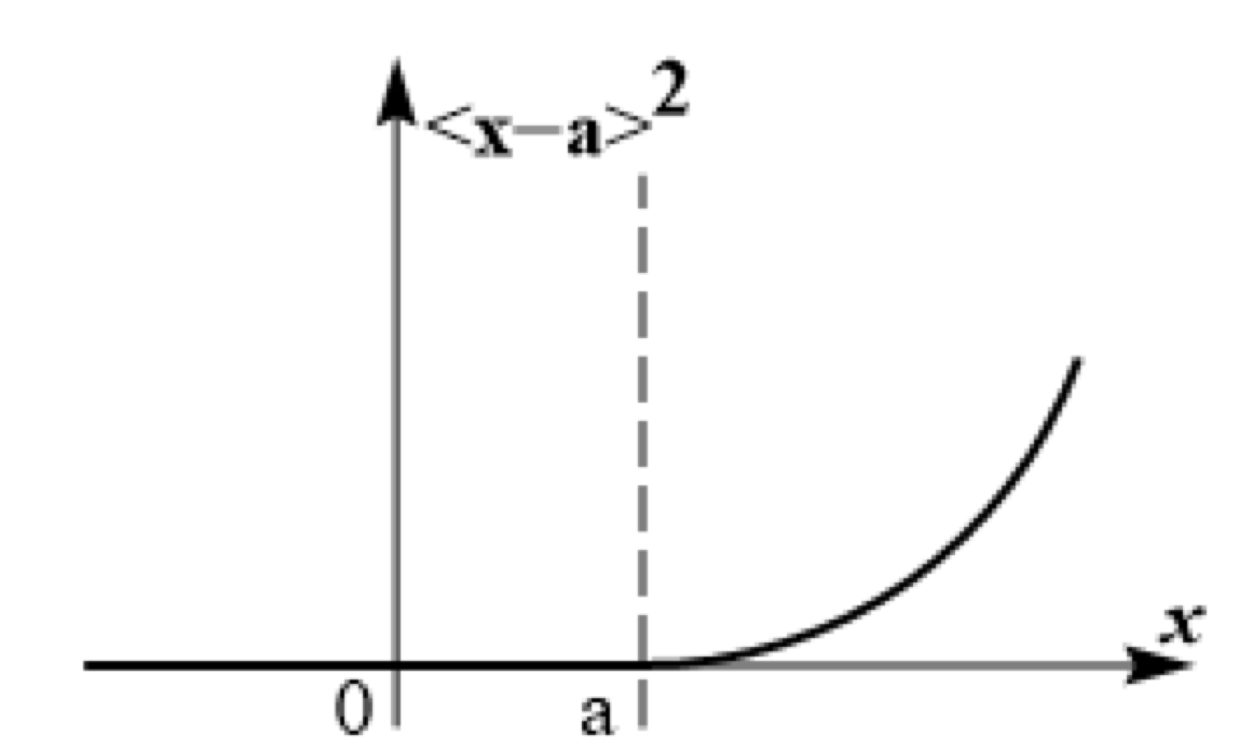
\includegraphics[width=.3\textwidth]{imgs/func_singul_2.jpeg}
        \end{minipage}  &
        \begin{minipage}{.4\textwidth}
            Também usado mais para análise de carregamento de vigas, mas nesse caso a força é zero até certo ponto $a$ e depois segue uma distribuição quadrática.
        \end{minipage}              \\ \hline

        $\langle x - a\rangle^{-1}$                                    &
        \begin{minipage}{.3\textwidth}
            \centering
            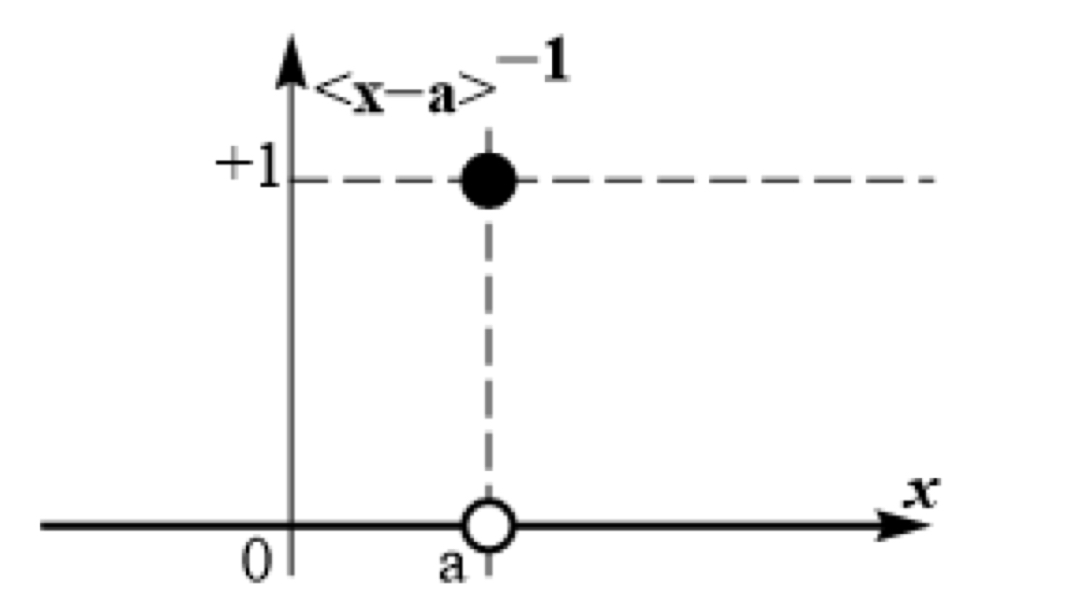
\includegraphics[width=.3\textwidth]{imgs/func_singul_-1.jpeg}
        \end{minipage} &
        \begin{minipage}{.4\textwidth}
            Usando bastante para representar forças pontuais durante análise de vigas, mas também usada para representar momentos durante análise de eixos.
        \end{minipage}                     \\ \hline

        $\langle x - a\rangle^{-2}$                                    &
        \begin{minipage}{.3\textwidth}
            \centering
            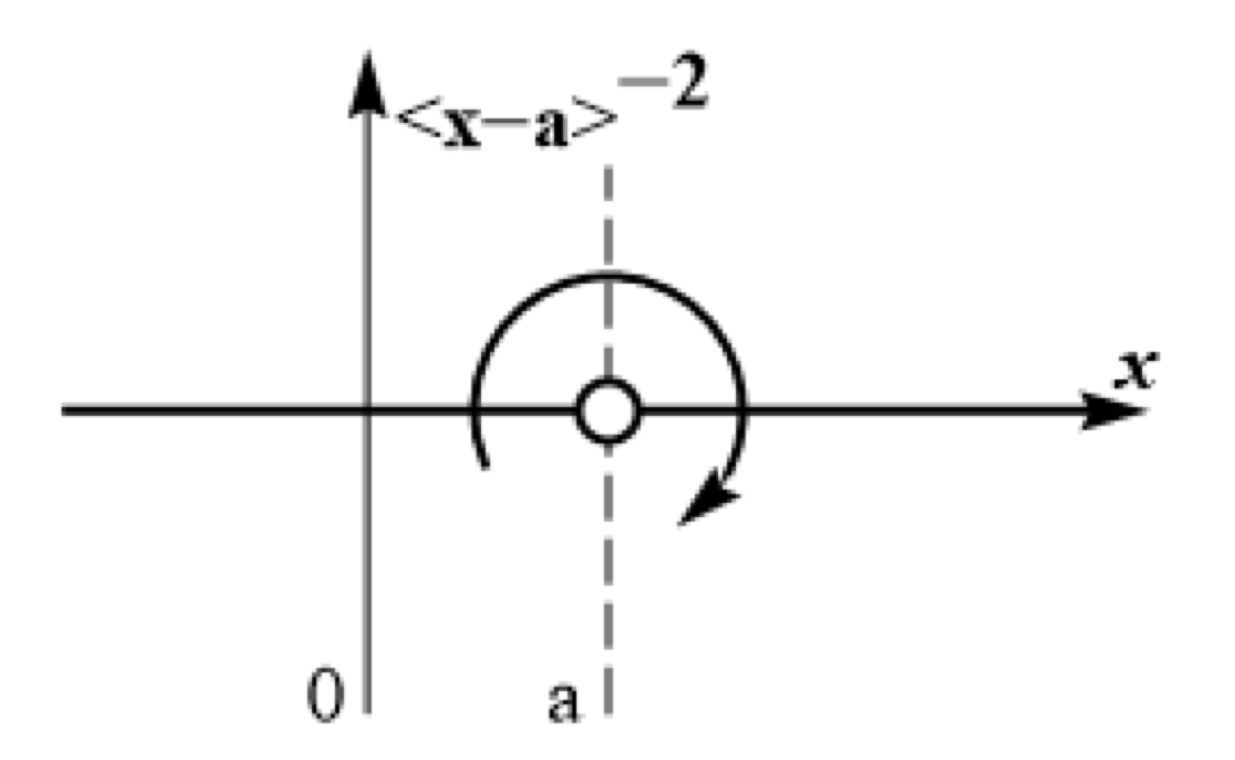
\includegraphics[width=.3\textwidth]{imgs/func_singul_-2.jpeg}
        \end{minipage} &
        \begin{minipage}{.4\textwidth}
            Usado bastante durante análise de vigas para representar momentos fletores.
        \end{minipage}                                                                                         \\ \hline
    \end{tabularx}
\end{table}

Integração de Função de Singularidade:

\begin{minipage}{\textwidth}\tiny
    \begin{align*}
        \int \langle x-a\rangle^m dx    & = \frac{\langle x - a \rangle ^{m+1}}{m + 1}, m \ge 0 \\
        \int \langle x-a\rangle^{-1} dx & = \langle x - a \rangle^0                             \\
        \int \langle x-a\rangle^{-2} dx & = \langle x - a \rangle^{-1}                          \\
    \end{align*}
\end{minipage}

\begin{minipage}[t]{.7\textwidth}
    Passo a Passo:
    \begin{enumerate}\addtocounter{enumi}{-1}\tiny
        \item Separar Carregamentos externos que são separáveis em seus respectivos modelos (barra, eixo, viga).
        \item Estabelecer uma convenção de sinais: A fim de padronizar, seguir a convenção da figura \ref{fig:conv_de_sinais_esf_intern}
        \item Estabelecer uma equação diferencial: A partir da tabela \ref{tb:edo_esf_internos}
        \item Descrever condições de Contorno e Restrição: Bom indicativo é começar pelos da tabela \ref{tb:cond_contorno} + Comportamento de Rótulas
        \item Integrar a equação diferencial: Como mostrado na subsection anterior
        \item Determinar Constantes de Integração: Substituindo os valores de contorno (já que são os únicos pontos conhecidos)
    \end{enumerate}
\end{minipage}\hfill
\begin{minipage}[t]{.3\textwidth}
    Check list:
    \begin{todolist}\tiny
        \item Não está esquecendo nenhuma força ?
        \item Modelou correto as forças de reação de cada suporte?
        \item Separou os tipos de load para cada modelo de corpo correto?
        \item Não adicionou forças de contorno na modelagem do load externo?
        \item Determinou as condições de contorno e de restrição necessárias?
    \end{todolist}
\end{minipage}


\section{Tensões e Deformações}
Veremos agora uma abordagem mais focada no estudo das tensões que certa estrutura está se submento, tendo em vista que durante o dimensionamento e o projeto das estruturas, o principal ponto de estudo são as tensões.

\subsection{Estado de Tensões}

\subsubsection*{Tensor de Tensões}

Vimos que em um corpo, existem dois tipos de tensões, as \textbf{Tensões Normais} $\sigma_{xx}$, que como o próprio nome indica seu vetor estão orientados paralelo ao vetor normal da superfície, e as \textbf{Tensões de Cisalhamento} $\sigma_{xy}$, que representam as tensões "deslisantes" em um corpo. A fim de representar todas as tensões (tanto normais quanto de cisalhamento) presentes em \emph{um ponto}, nós utilizamos um  \textbf{Tensor de Tensões} (também chamado de Estado de tensões), que nada mais é que um tensor \footnote{Um tensor é uma matriz que possui certas propriedades matemáticas, \emph{e.g} mudança de coordenadas mantém significado físico} como mostrado abaixo:

$$$$
\begin{minipage}{.5\textwidth}
    \begin{align*}
        \sigma = \begin{vmatrix}
                     \sigma_{XX} & \sigma_{XY} & \sigma_{XZ} \\
                     \sigma_{YX} & \sigma_{YY} & \sigma_{YZ} \\
                     \sigma_{ZX} & \sigma_{ZY} & \sigma_{ZZ}
                 \end{vmatrix}
    \end{align*}
\end{minipage}
\begin{minipage}{.5\textwidth}
    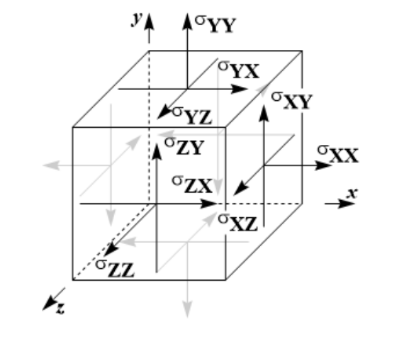
\includegraphics[width=.5\textwidth]{imgs/tensões.png.png}
\end{minipage}
$$$$

Algo de suma importância de ser ressaltado é a \textbf{Simetria} do tensor de tensão, onde $\sigma_{ZX} = \sigma_{XZ}$, e assim por diante. Além disso, temos que a diagonal principal da matriz representa as tensões normais.

Tal tensor, pode ainda ser simplificado nso casos de \emph{Estado plano de Tensões}, onde o tensor é reduzido para uma matriz $2x2$ (um problema $2D$) quando as tensões com componentes $z$ são nulas (\emph{e.g} estudo de tensões em fuselagem e avião), como mostrado abaixo:

$$$$
\begin{minipage}{.5\textwidth}
    \begin{align*}
        \sigma = \begin{vmatrix}
                     \sigma_{XX} & \sigma_{XY} \\
                     \sigma_{YX} & \sigma_{YY}
                 \end{vmatrix}
    \end{align*}
\end{minipage}
\begin{minipage}{.5\textwidth}
    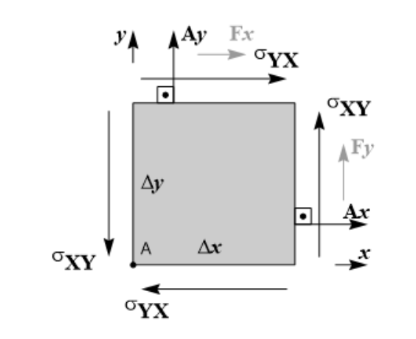
\includegraphics[width=.5\textwidth]{imgs/2d_tens.png}
\end{minipage}
$$$$

Uma observação importante de ser feita é que a tensão é dad apor $F/A$ para os casos onde as forças sendo aplicadas são uniformes, então as tensões de cisalhamento são dadas pelas forças paralela a face da superficie dividada pela área da superfície, e a anlogamenta a tensão normal é a força normal à face sobre a área da face. Como podemos ver na imagem acima e descrito pela equação abaixo:
\begin{align*}
    \sigma_{XX} & = F_{N_X} / A_x \\
    \sigma_{YY} & = F_{N_Y} / A_y \\
                & .               \\ &. \\ &.
\end{align*}

\newpage
\subsubsection*{Círculo de Mohr}
Acabamos de ver que para cada ponto em um corpo há um tensor de tensões que repesenta todas as tensões que um corpo está sofrendo. Como as tensões são cisalhantes e normais, o ângulo no qual estamos analisando o ponto influencia nos valores de cada tipo de tensão. Quando analisamos, entretanto, vemos que para um ponto qualquer, a análise dos valores das tensões normais e cisalhantes sob qualquer ângulo de análise ($0^\circ \le \theta \le 360^\circ $) caem sobre um circulo, chamado de \textbf{Circulo de Morh}.

No círculo de Mohr nós temos no eixo $x$ o valor das tensões normais e no eixo $y$ o valor das tensões cisalhantes. Possuindo como centro e raio:
\begin{align*}
    X_0 = \frac{\sigma_{XX} + \sigma_{YY}}{2}, R = \sqrt{\left(\frac{\sigma_{XX} - \sigma_{YY}}{2}\right)^2 + \sigma^2_{XY}}
\end{align*}

Nós utilizamos esse circulo para calcular, a partir de uma orientação com as tensões conhecidas, os novos valores de tensões de cisalhamento e normais para qualquer nova orientação, pois existe uma relação entre o angulo entre a nova orientação e a orientação original $\theta_{real}$ e o angulo a ser analisado no circulo $\theta_{circ}$, onde $\theta_{circ} = -2\theta_{real}$, isso é, para um angulo $\theta_{real}$ entre a orientação de análise conhecida e a nova face de estudo, nós analisamos no circulo de Mohr um ponto que está a duas vezes $\theta_{real}$, mas no sentido contrário, como podemos ver pela imagem abaixo:
\begin{figure}[h]
    \centering
    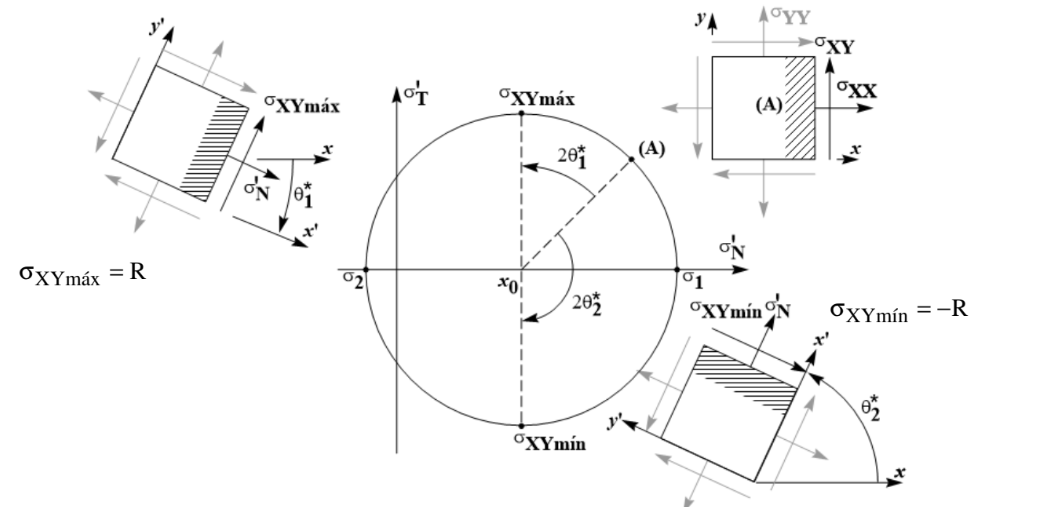
\includegraphics[width=.8\textwidth]{imgs/cir_mohr.png}
\end{figure}

Ser capaz de analisar os novos valores das tensões normais e de cisalhamento é importante pois certo materiais não são capazes de sustentar tensões normais de forma eficiente, o que pode levar a sua fadiga. Por isso denominamos a orientação com o maior valor de tensão normal ($ \sigma_{n_{max}} = X_0 + R$) de \textbf{plano principal}. Além disso temos também os \textbf{Planos de Cisalhamento Máximo} que, como a origem do circulo está sempre no eixo $x$ (eixo das tensões normais), possui o valor máximo de tensão de cisalhamento igual a $R$ (igual ao raio do circulo).

Para facilitar a solução de problemas através do circulo de Morh temos o seguinte passo a passo:
\begin{enumerate}
    \item \textbf{Montar Tensor de Tensão}: Como dito anteriormente, somos capazes de ver cada componente da tensão a partir da relação $F/A$ a partir das forças e áreas relacionadas.
    \item \textbf{Calculo de Centro}: Calcular o centro do circulo a partir das tensões normais.
    \item \textbf{Calculo de Raio}: Calcular o raio do circulo.
    \item \textbf{Desenhar o Circulo}: Desenhar com os eixos corretos, com o centro e valores máximos e mínimos corretos.
    \item \textbf{Desenhar Corpo a ser Analisado}: Nós fazemos o circulo a partir de uma posição conhecida (consideramos essa posição $\theta=0$), e é necessário desenhar o corpo na nova posição a ser analisado para facilitar a identificação do ângulo do plano $\theta_{target}$
    \item \textbf{Análise do Circulo}: Analisar o ponto $\theta_{circ} = -2 \theta_{target}$
\end{enumerate}

\subsection{Estado de Deformação}
Deformações sofridas por estruturas podem ser descritas de diferentes formas, considerando somente deformações axiais, contínuas ou ainda angulares. A forma que iremos abordar é a mais generalista, chamada de \textbf{Estado Geral de Deformação}, que assim como o Estado geral de tensões é representado por um \emph{tensor}, mostrado abaixo:
\begin{align*}
    \varepsilon =  \begin{bmatrix}
                       \varepsilon_{XX} & \varepsilon_{XY} & \varepsilon_{XZ} \\
                       \varepsilon_{YX} & \varepsilon_{YY} & \varepsilon_{YZ} \\
                       \varepsilon_{ZX} & \varepsilon_{ZY} & \varepsilon_{ZZ}
                   \end{bmatrix}
    \Rightarrow \varepsilon_{ij} = \frac{1}{2}\left(\frac{du_i}{dx_j}+\frac{du_j}{dx_i}\right)
\end{align*}

Onde, utilizando como exemplo $\varepsilon_{XY}$, temos $i=1, j=2$ e $\varepsilon_{XY} = 1/2\left(\frac{du}{dy} + \frac{dv}{dx}\right)$. A partir desse exemplo podemos ver que que estamos compondo o tensor com a soma das derivadas da deformação $\{u, v, w\}$, chamada de \textbf{campo de deslocamento}, em relação as coordenadas $\{x, y, z\}$. Logo quando falamos $u_i$ estamos falando da $i-esima$ componente do campo de deslocamento e quando falamos $x_j$ estamos falando a $j-esima$ coordenada (onde no nosso exemplo se temos $i=1$ estamos falando da primeira componente ($u$) do campo de deslocamento, e com $j=2$ estamos falando da segunda coordenada o ($y$)).

Uma outra forma de calcular o estado de deformação, para o caso específico de \textbf{Deformação Térmica}, é:
\begin{align*}
    \varepsilon_T = \alpha \Delta T
\end{align*}

Onde temos $\alpha$ como o calor específico e $\Delta T$ a variação de temperatura. A partir disso, somos capazes de calcular a deformação total através da seguinte derivada (para o caso 2D de expansão térmica):
\begin{align*}
    \delta = \int^L_0 \varepsilon_T dx
\end{align*}

\subsection{Equação Constitutiva}
A partir de agora iremos ligar as partes anteriores desse capitulo e investigar a relação entre as tensões sofridas por um corpo e sua deformação.

Tal relação, após inúmeros testes, foi descoberta ser dependente do material. De forma geral, a relação entre tensão e deformação é dada por:
\begin{align*}
    \begin{Bmatrix}
        \sigma_{XX} \\
        \sigma_{YY} \\
        \sigma_{ZZ} \\
        \sigma_{YZ} \\
        \sigma_{XZ} \\
        \sigma_{XY} \\
    \end{Bmatrix} =
    \begin{bmatrix}
        c_{11} & c_{12} & c_{13} & c_{14} & c_{15} & c_{16} \\
        c_{21} & c_{22} & c_{23} & c_{24} & c_{25} & c_{26} \\
        c_{31} & c_{32} & c_{33} & c_{34} & c_{35} & c_{36} \\
        c_{41} & c_{42} & c_{43} & c_{44} & c_{45} & c_{46} \\
        c_{51} & c_{52} & c_{53} & c_{54} & c_{55} & c_{56} \\
        c_{61} & c_{62} & c_{63} & c_{64} & c_{65} & c_{66}
    \end{bmatrix}
    \begin{Bmatrix}
        \varepsilon_{XX}  \\
        \varepsilon_{YY}  \\
        \varepsilon_{ZZ}  \\
        2\varepsilon_{YZ} \\
        2\varepsilon_{XZ} \\
        2\varepsilon_{XY} \\
    \end{Bmatrix}
\end{align*}

Onde a matriz $C\Rightarrow c_{ij}$ é composta por 36 propriedades do material em questão. Sendo que a depender do material e do seu tipo esse número pode ser menor devido a simetria entre outras coisas.

A partir disso, podemos classificar os diferentes materiais a depender do seu grau de simetria:




\end{document}